
Let the number of toys of type A be $x$ and the number of toys of type B be $y$  such that 
\begin{align}
    x \geq 0 \\
    y \geq 0 
\end{align}
According to the question,
\begin{align}
    12x+6y &\leq 360 \\
    \implies 2x+y &\leq 60 
\end{align}
and,
\begin{align}
    18x+0y &\leq 360 \\
    \implies x &\leq 20
\end{align}
and,
\begin{align}
     6x+9y &\leq 360 \\
    \implies 2x+3y &\leq 120 
\end{align}
$\therefore$ Our problem is
\begin{align}
        \max_{\vec{x}} Z &= \myvec{7.5 & 5}\vec{x}\\
        s.t. \quad 
        \myvec{2 & 1 \\ 1 & 0 \\2 & 3 }\vec{x} &\preceq \myvec{60\\20\\120} 
\end{align}
Lagrangian function is given by
\begin{equation}
\begin{aligned}
    &L(\vec{x},\boldsymbol{\lambda}) \\ &= \myvec{7.5 & 5}\vec{x}+\lcbrak{\sbrak{\myvec{2 & 1}\vec{x}-60}} \\ &+ \sbrak{\myvec{1 & 0}\vec{x}-20} +\sbrak{\myvec{2 & 3}\vec{x}-120} \\ &+ \sbrak{\myvec{-1 & 0}\vec{x}} +\rcbrak{\sbrak{\myvec{0 & -1}\vec{x}}}\boldsymbol{\lambda}
\end{aligned}
\end{equation}
where,
\begin{align}
    \boldsymbol{\lambda} &= \myvec{\lambda_1 \\ \lambda_2 \\ \lambda_3 \\ \lambda_4 \\ \lambda_5 \\ \lambda_6}
\end{align}
Now,
\begin{align}
    \nabla L(\vec{x},\boldsymbol{\lambda}) &= \myvec{7.5+ \myvec{2 & 1 & 2 & -1 & 0 }\boldsymbol{\lambda}\\ 5+\myvec{1 & 0 & 3 & 0 & -1}\boldsymbol{\lambda} \\ \myvec{2 & 1}\vec{x}-60 \\ \myvec{1 & 0}\vec{x}-20 \\ \myvec{2 & 3}\vec{x}-120 \\ \myvec{-1 & 0}\vec{x} \\ \myvec{0 & -1}\vec{x}}
\end{align}
$\therefore$ Lagrangian matrix is given by
\begin{align}
    \myvec{0 & 0 & 2 & 1 & 2 & -1 & 0 \\ 0 & 0 & 1 & 0 & 3 & 0 & -1 \\ 2 & 1 & 0 & 0 & 0 & 0 & 0 \\ 1 & 0 & 0 & 0 & 0 & 0 & 0 \\ 2 & 3 & 0 & 0 & 0 & 0 & 0 \\ -1 & 0 & 0 & 0 & 0 & 0 & 0 \\ 0 & -1 & 0 & 0 & 0 & 0 & 0 }\myvec{\vec{x} \\ \boldsymbol{\lambda} } &= \myvec{-7.5 \\ -5 \\ 60 \\ 20 \\ 120 \\ 0 \\0 }
\end{align}
Considering $\lambda_1,\lambda_2$ as only active multiplier,
\begin{align}
    \myvec{0 & 0 & 2 & 2 \\ 0 & 0 & 1 & 3 \\ 2 & 1 & 0 & 0 \\ 2 & 3 & 0 & 0}\myvec{\vec{x}\\ \boldsymbol{\lambda}} &= \myvec{-7.5 \\ -5 \\ 60 \\ 120}
\end{align}
resulting in,
\begin{align}
    \myvec{\vec{x} \\ \boldsymbol{\lambda}} &= \myvec{0 & 0 & 2 & 2 \\ 0 & 0 & 1 & 3 \\ 2 & 1 & 0 & 0 \\ 2 & 3 & 0 & 0}^{-1}\myvec{-7.5 \\ -5 \\ 60 \\ 120}
    \\
    \implies   \myvec{\vec{x} \\ \boldsymbol{\lambda}} &= \myvec{0 & 0 & \frac{3}{4} & \frac{-1}{4} \\ 0 & 0 & \frac{-1}{2} & \frac{1}{2} \\ \frac{3}{4} & \frac{-1}{2} & 0 & 0 \\ \frac{-1}{4} & \frac{1}{2} & 0 & 0}\myvec{-7.5 \\ -5 \\ 60 \\ 120}
    \\
    \implies \myvec{\vec{x} \\ \boldsymbol{\lambda}} &= \myvec{15 \\ 30 \\ -3.125 \\ -0.625}
\end{align}
$\because \boldsymbol{\lambda}=\myvec{-3.125 \\ -0.625} \succ \vec{0} $
\\
$\therefore$ Optimal solution is given by
\begin{align}
    \vec{x} &= \myvec{15\\30} \\
    Z &= \myvec{7.5 & 5}\vec{x} \\
    &= \myvec{7.5 & 5}\myvec{15 \\ 30} \\
    &= 262.5
\end{align}
By using cvxpy in python ,
\begin{align}
    \vec{x}=\myvec{14.99999998\\29.99999996}\\
    Z = 262.49999967
\end{align}
Hence, the manufacturer should manufacture \boxed{x=15} toys of type A and \boxed{y=30} toys of type B in a day to get maximum profit \boxed{Z=\text{Rs} 262.5}.
This can be verified in Fig. \ref{opt/26/fig:toy problem}	
\begin{figure}[!ht]
\centering
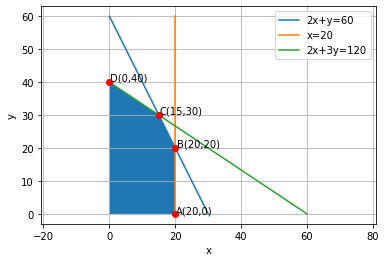
\includegraphics[width=\columnwidth]{solutions/su2021/2/26/Figure10.png}
\caption{Toy Problem}
\label{opt/26/fig:toy problem}	
\end{figure}
